% This is the Reed College LaTeX thesis template. Most of the work
% template. Later comments etc. by Ben Salzberg (BTS). Additional
% restructuring and APA support by Jess Youngberg (JY).
% Your comments and suggestions are more than welcome; please email
% them to cus@reed.edu
%
% See http://web.reed.edu/cis/help/latex.html for help. There are a
% great bunch of help pages there, with notes on
% getting started, bibtex, etc. Go there and read it if you're not
% already familiar with LaTeX.
%
% Any line that starts with a percent symbol is a comment.
% They won't show up in the document, and are useful for notes
% to yourself and explaining commands.
% Commenting also removes a line from the document;
% very handy for troubleshooting problems. -BTS

% As far as I know, this follows the requirements laid out in
% the 2002-2003 Senior Handbook. Ask a librarian to check the
% document before binding. -SN

%%
%% Preamble
%%
% \documentclass{<something>} must begin each LaTeX document
\documentclass[12pt,twoside]{reedthesis}
% Packages are extensions to the basic LaTeX functions. Whatever you
% want to typeset, there is probably a package out there for it.
% Chemistry (chemtex), screenplays, you name it.
% Check out CTAN to see: http://www.ctan.org/
%%
\usepackage{graphicx,latexsym}
\usepackage{amsmath}
\usepackage{amssymb,amsthm}
\usepackage{longtable,booktabs,setspace}
\usepackage{chemarr} %% Useful for one reaction arrow, useless if you're not a chem major
\usepackage{rotating}

% Modified by CII
\usepackage[hyphens]{url}
\usepackage{hyperref}
\usepackage{lmodern}

% Added by CII (Thanks, Hadley!)
% Use ref for internal links
\renewcommand{\hyperref}[2][???]{\autoref{#1}}
\def\chapterautorefname{Chapter}
\def\sectionautorefname{Section}
\def\subsectionautorefname{Subsection}

\usepackage{caption}
\captionsetup{width=5in}

% \usepackage{times} % other fonts are available like times, bookman, charter, palatino

\title{My Final College Paper}
\author{Philip Stallworth}
% The month and year that you submit your FINAL draft TO THE LIBRARY (May or December)
\date{May 2026}
\division{Mathematics and Natural Sciences}
\advisor{Andrew Bray}
%If you have two advisors for some reason, you can use the following
%\altadvisor{Your Other Advisor}
%%% Remember to use the correct department!
\department{Mathematics}
% if you're writing a thesis in an interdisciplinary major,
% uncomment the line below and change the text as appropriate.
% check the Senior Handbook if unsure.
%\thedivisionof{The Established Interdisciplinary Committee for}
% if you want the approval page to say "Approved for the Committee",
% uncomment the next line
%\approvedforthe{Committee}

% Below added by CII

%%% Copied from knitr
%% maxwidth is the original width if it's less than linewidth
%% otherwise use linewidth (to make sure the graphics do not exceed the margin)
\makeatletter
\def\maxwidth{ %
  \ifdim\Gin@nat@width>\linewidth
    \linewidth
  \else
    \Gin@nat@width
  \fi
}
\makeatother

\renewcommand{\contentsname}{Table of Contents}

\setlength{\parskip}{0pt}

\providecommand{\tightlist}{%
  \setlength{\itemsep}{0pt}\setlength{\parskip}{0pt}}

\Acknowledgements{
I want to thank a few people.
}

\Dedication{
You can have a dedication here if you wish.
}

\Preface{
This is an example of a thesis setup to use the reed thesis document
class.
}

\Abstract{
``The preface pretty much says it all.''
}


%%
%% End Preamble
%%
%

\begin{document}

      \maketitle
  
  \frontmatter % this stuff will be roman-numbered
  \pagestyle{empty} % this removes page numbers from the frontmatter

      \begin{acknowledgements}
      I want to thank a few people.
    \end{acknowledgements}
  
      \begin{preface}
      This is an example of a thesis setup to use the reed thesis document
      class.
    \end{preface}
  
  % Add table of abbreviations?

      \hypersetup{linkcolor=black}
    \setcounter{tocdepth}{2}
    \tableofcontents
  
      \listoftables
  
      \listoffigures
  
      \begin{abstract}
      ``The preface pretty much says it all.''
    \end{abstract}
  
      \begin{dedication}
      You can have a dedication here if you wish.
    \end{dedication}
  
  \mainmatter % here the regular arabic numbering starts
  \pagestyle{fancyplain} % turns page numbering back on

  \chapter*{Introduction}\label{introduction}
  \addcontentsline{toc}{chapter}{Introduction}
  
  Spatial point patterns, data in the form of a set of points on the
  plane, emerge frequently in practice. Their remarkable theoretical
  properties permit a surprisingly unified study of data as seemingly
  disparate as the locations of stars in the sky, the dispersal of trees
  in a forest, and the occurrences of crime in a neighborhood.
  
  As a simple illustration, figure 1 presents the locations of trees in a
  New Zealand forest plot. Each point represents a tree and its location
  represents its position in an approximately 140 by 85 foot forest plot.
  These data were gathered from a complete sampling of the forest plot and
  do not contain additional information on the underlying features of the
  land quality, the type of tree, or the size of the tree. The uninformed
  statistician must proceed through inference solely based upon these
  events, their locations in the plot, and their locations relative to one
  another. This is actually a remarkably rich amount of information.
  Statistical models can detect clustering, regularity, variation in the
  underlying region, and event intensity. However, many methods rely on
  sampling that accounts for every event in an area. This form of sampling
  is often expensive, time-consuming, and error prone.
  
  Cheaper, less time-consuming sampling methods exist. One in particular,
  T-square sampling, has a rich theoretical literature which has found
  methods for detecting clustering and regularity. In this thesis, I hope
  to expand the, rather empty, corpus on an even simpler sampling scheme:
  k-trees sampling.
  
  K-tree sampling schemes find the k-nearest events to points specified in
  a pre-determined array. Little research has been done to determine how
  clustering and regularity could be detected under such a sampling
  scheme. This is because of the inability to reliably compute point to
  point nearest neighbors with incomplete sampling. I do not try and
  resolve this issue. Instead, I work with a number of datasets containing
  data collected through the 1-tree sampling of the same plant in a number
  of bogs. I assume both that there are two sources of clustering, event
  based and underlying region based, and that event based clustering is
  consistent from dataset to dataset, while underlying region clustering
  varies. We can then incorporate event based clustering mechanisms into
  future models of the same process.\\
  
  \begin{figure}
  
  {\centering 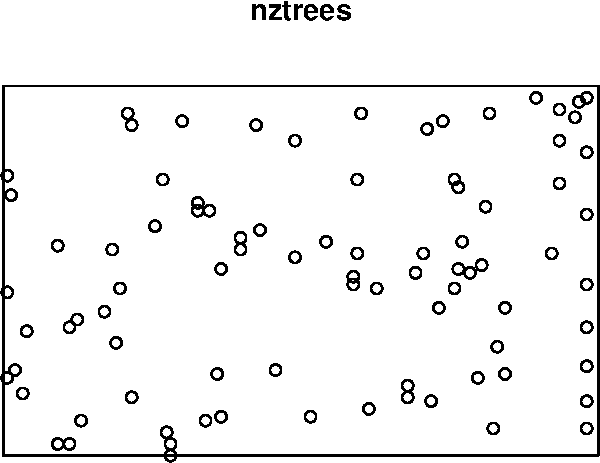
\includegraphics{Draft_files/figure-latex/fig1-1} 
  
  }
  
  \caption[Caption]{Caption}\label{fig:fig1}
  \end{figure}
  
  \chapter{Spatial Point Processses and the Poisson
  Process}\label{rmd-basics}
  
  \section{Informal Definitions and
  Comments}\label{informal-definitions-and-comments}
  
  A \emph{spatial point process}, subsequently referred to as a point
  process, is a stochastic mechanism which generates a countable set of
  events in the plane (\(\mathbb{R}^2\)). Simple point processes are
  typically \emph{stationary} and \emph{isotropic}. The properties of a
  stationary point process are invariant under translation, while the
  properties of an isotropic point process are invariant under rotation.
  These definitions are less restrictive than they might seem. For
  instance, they allow for random heterogeneity in the underlying
  environment. Though defined over the entire plane, spatial point
  processes are only applied to data from finite regions. Furthermore, in
  practice, models assuming isotropy or stationarity are typically
  appropriate for point processes that exhibit approximate stationarity or
  isotropy.
  
  Statistical analyses of spatial point pattern data typically involve
  comparisons between empirical summary descriptions of the data and the
  corresponding theoretical summary descriptions of a model. Importantly,
  these theoretical summary descriptions must be derived from an
  underlying model, rather than being models themselves. The most common
  comparisons pit the empirical summary descriptions against the
  corresponding summary description under a homogeneous Poisson process.
  For a more complete introduction to spatial point processes see either
  Moller and Waagepetersen's \emph{Statistical Inference and Simulation
  for Spatial Point Processes} or Diggle's \emph{Statistical Analysis of
  Spatial Point Patterns}.
  
  \section{Point Processes}\label{point-processes}
  
  A \emph{spatial point process} \(X\) is a random countable subset of a
  space \(S\). In this thesis, \(S\) will always be a subset of
  \(\mathbb{R}^d\) and \(d\) will typically be 2. Often \(S\) will either
  be a \(d\)-dimensional box or all of \(\mathbb{R}^d\). In practice, we
  only observe the points in an observation window \(W\subseteq S\).
  
  I restrict my attention to point processes \(X\) whose realizations are
  locally finite subsets of \(S\). For any subset \(x\subset S\), let
  \(n(x)\) denote the cardinality of \(x\), setting \(n(x) = \infty\) if
  \(x\) is not finite. \(x\) is said to be \emph{locally finite}, if
  \(n(x_B)\) is finite whenever \(B\subset S\) is bounded, where
  \[x_B = x \cap B \] is the restriction of a point configuration \(x\) to
  \(B\). Consequently, \(X\) takes values in the space defined by
  \[N_{lf} = \{ x\subseteq S | n(x_B) < \infty \text{ for all bounded } B\subseteq S \}.\]
  
  Elements of \(N_{lf}\) are called \emph{locally finite point
  configurations}, and they will be denoted by \(x, y, \dots\) while
  \(\xi, \eta, \dots\) will denote points in \(S\). I will typically write
  \(x\cup \xi\) for \(x\cup \{ \xi \}\), \(x\setminus \eta\) for
  \(s\setminus \{\eta\}\), when \(x\in N_{lf}\) and \(\xi, \eta \in S\).
  
  \section{Poisson Point Processes}\label{poisson-point-processes}
  
  The Poisson process plays a central role in the point process
  literature. It serves as the tractable model for ``completely spatially
  random'' point processes. Real processes which exhibit complete spatial
  randomness are undoubtedly rare. However, by comparing empirical summary
  statistics to those under a theoretical Poisson, statisticians and
  scientists are able to detect clustering, regularity, and inhomogeneity
  in the underlying environments. Researchers typically begin data
  analysis with these comparisons.
  
  \subsection{Basic Properties}\label{basic-properties}
  
  First, lets consider a Poisson point process defined on a space
  \(S\subseteq \mathbb{R}^d\) and specified by a \emph{intensity functon}
  \(\rho : S \rightarrow [0, \infty]\) which is \emph{locally integrable},
  i.e. \(\int_B \rho(\xi) d\xi < \infty\) for all bounded
  \(B\subseteq S\). For the following definition, we use the
  \emph{intensity measure} \(\mu\) defined by
  \[\mu(B) = \int_B \rho(\xi) d\xi, \; \; B\subseteq S.\] Clearly, this
  measure is locally finite. It is also \emph{diffuse}, i.e.
  \(\mu (\{ \xi \}) = 0\) for all \(\xi \in S\).
  
  \textbf{Definition:} Let \(f\) be a density function on a set
  \(B\subseteq S\), and let \(n\in \mathbb{N}\). A point process \(X\)
  consisting of \(n\) points in \(B\) with density \(f\) is called a
  \emph{binomial point process} of \(n\) points in \(B\) with density
  \(f\). We write \(X\sim \text{binomial}(B, n, f)\).
  
  \textbf{Definition:}A point process \(X\) on \(S\) is a \emph{Poisson
  point process} with intensity function \(\rho\) if the following
  properties are satisfied:
  
  \begin{enumerate}
  \def\labelenumi{\arabic{enumi}.}
  \itemsep1pt\parskip0pt\parsep0pt
  \item
    For any \(B\subseteq S\) with \(\mu(B) < \infty\),
    \(N(B) \sim \text{poisson}(\mu(B))\), the Poisson distribution with
    mean \(\mu(B)\).
  \item
    For any \(n\in \mathbb{N}\) and \(B\subseteq S\) with
    \(0\leq \mu(B) < \infty\), conditional on \(N(B) = n\),
    \(X_B \sim \text{binomial}(B, n, F)\) with
    \(f(\xi) = \rho(\xi) / \mu(B)\) We then write
    \(X \sim \text{Poisson}(S, \rho)\).
  \end{enumerate}
  
  Sometimes (ii) is replaced with the condition that
  \(N(B_1), N(B_2), \dots N(B_n)\) are independent for disjoint sets
  \(B_1, B_2, \dots, B_n \subseteq S\) and \(n\geq 2\). This is called
  \emph{independent scattering}. Consequently, \(\mu\) determines the
  expected number of points in any \(B\subseteq S\). \(\rho(\xi) d\xi\)
  can be thought of as the probability for the occurrence of an event in
  an infinitesimally small ball with center \(\xi\) and volume \(d\xi\).
  
  \textbf{Definition:} If \(\rho\) is constant, the process
  Poisson(\(S, \rho\)) is called a \emph{homogeneous Poisson process} on
  \(S\) with \emph{rate} or \emph{intensity} \(\rho\); otherwise it is an
  \emph{inhomogeneous Poisson process} on \(S\).
  
  Figure 1.1 displays examples of both homogeneous and inhomogeneous
  Poisson processes. It should be clear why the homogeneous poisson
  process matches notions of complete spatial randomness. Homogeneous
  Poisson processes are both stationary and isotropic.
  
  \textbf{Definition:} A point process \(X\) on \(\mathbb{R}^d\) is
  \emph{stationary} if its distribution is translation invariant. In other
  words, if the distribution of \(X + s = \{\xi + s: \xi\in X\}\) is the
  same as \(X\) for any \(s\in \mathbb{R}^d\). \(X\) is \emph{isotropic}
  if its distribution is rotation invariant about the origin.
  
  \begin{figure}
  
  {\centering 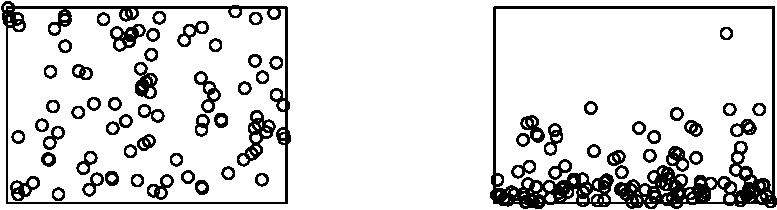
\includegraphics{Draft_files/figure-latex/fig1_1-1} 
  
  }
  
  \caption[Caption]{Caption}\label{fig:fig1_1}
  \end{figure}
  
  The following expansion is often useful.
  
  \textbf{Proposition 1.1:}
  
  \begin{enumerate}
  \def\labelenumi{(\roman{enumi})}
  \itemsep1pt\parskip0pt\parsep0pt
  \item
    \(X\sim \text{Poisson}(S, \rho)\) if and only if for all
    \(B\subseteq S\) with \(\mu(B) = \int_S \rho(\xi) d\xi < \infty\) and
    all \(F\subseteq N_{lf}\),
    \[P(X_B\in F) = \sum_{n = 0}^\infty \frac{exp(-\mu(B))}{n!} \int_B \cdots \int_B \mathbf{1}[\{x_1, x_2, \dots, x_n\} \in F] \prod_{i = 1}^n \rho(x_i)dx_1dx_2 \dots dx_n\]
    where the integral for \(n = 0\) is \(\mathbf{1} [\emptyset \in F].\)
  \item
    If \(X\sim \text{Poisson}(S, \rho)\), then for functions
    \(h:N_{lf} \rightarrow [0, \infty)\) and \(B\subseteq S\) with
    \(\mu(B) < \infty\),
    \[\mathbb{E} [h(X_B)] = \sum_{n = 0}^\infty \frac{exp(-\mu(B))}{n!} \int_B \cdots \int_B h(\{x_1, \dots, x_n \}) \prod_{i = 1}^n dx_1\cdots dx_n.\]
  \end{enumerate}
  
  A second proposition demonstrates the validity of the independent
  scattering property of Poisson processes.
  
  \textbf{Proposition 1.2:} If \(X\) is a Poisson process on \(S\), then
  \(X_{B_1}, X_{B_2}, \dots\) are independent for disjoint sets
  \(B_1, B_2, \dots \subseteq S\).
  
  Proof: Suppose \(X\) is a Poisson process on \(S\) and lets
  \(B_1, \dots, B_n \subseteq S\) be disjoint where \(n\geq 2\). First,
  suppose \(n = 2\). \textbf{IN PROGRESS}
  
  \subsubsection{Void Events}\label{void-events}
  
  The following discussion presents an alternative way to think of
  determining spatial point processes. Let
  \[ \mathcal{B}_0 = \{B \in \mathcal{B} : B \text{ is bounded}\}, \]
  where \(\mathcal{B}\) is the Borel \(\sigma\)-algebra. For a point
  process \(X\) on \(S\) let the \emph{count function} \[N(B) = n(X_B)\]
  be the random number of points falling in \(B\subseteq S\). Sets of the
  form \(F_B = \{x\in N_{lf}: n(x_B) = 0\}\) with \(B\in \mathcal{B}_0\)
  are called \emph{void events}. Clearly, \(X\in F_B\) if and only if
  \(N(B) = 0\). With some loose restrictions, the \emph{distribution} of
  \(X\) is determined by its \emph{void probabilities} defined by
  \[ \nu (B) = P(N(B)= 0), \; B\in \mathcal{B}_0\]
  
  The following theorem provides an alternative characterization of a
  Poisson process using void probabilities.
  
  \textbf{Theorem 1.1:} \(X\sim \text{Poisson}(S, \rho)\) exists and is
  determined by its void probabilities
  \[\nu(B) = \text{exp}(-\mu(B)), \; \; \text{bounded }B\subseteq S. \]
  
  \emph{Proof} Let \(\xi \in S\) be arbitrary and let
  \(B_i = \{ \eta \in S : i - 1 \leq ||\eta - \xi || < i \}\) for
  \(i \in \mathbb{N}.\) \(S\) is clearly a disjoint union of the bounded
  \(B_i\), where \(i\) is a non-zero natural number. Let
  \(X = \cup_1^\infty X_i\) where
  \(X_i \sim \text{Poisson}(B_i, \rho_i)\), are independent and where
  \(\rho_i\) is the restriction of \(\rho\) to \(B_i\). Then for bounded
  \(B\subseteq S\), \[
  \begin{aligned}
  P(X\cap B = \emptyset) &= \prod_{i = 1}^\infty P(X_i \cap B = \emptyset) = \prod_{i = 1}^\infty \text{exp}(-\mu(B\cap B_i))\\
  &= \text{exp}(\sum_{i=1}^\infty -\mu(B\cap B_i)) = \text{exp}(-\mu(B))
  \end{aligned}
  \] The final equality is the void probability for a Poisson process with
  intensity measure \(\mu\). Furthermore, it can be shown, but will not be
  shown here, that this characterization is unique.
  
  \subsection{Superpositioning and
  Thinning}\label{superpositioning-and-thinning}
  
  What follows are two operations for point processes. They will be an
  especially important tool for model fitting later in the thesis.
  
  \textbf{Definition:} A disjoint union \(\cup_{i = 1}^\infty X_i\) of
  point processes \(X_1, X_2, \dots\) is called a \emph{superposition}.
  
  \textbf{Definition:} Let \(p:S\rightarrow [0, 1]\) be a function and
  \(X\) a point process on \(S\). The point process
  \(X_{\text{thin}} \subseteq X\) obtained by including \(\xi \in X\) in
  \(X_{\text{thin}}\) with probability \(p(\xi)\), where points are
  included/excluded independently of each other, is said to be an
  \emph{independent thinning} of \(X\) with \emph{retention probabilities}
  \(p(\xi)\), \(\xi \in S\). Formally,
  \[ X_{\text{thin}} = \{ \xi \in X: \mathcal{R}(\xi) \leq p(\xi) \} \]
  where \(\mathcal{R}(\xi) \sim \text{Uniform}[0,1]\), \(\xi \in S\), are
  mutually independent and independent of \(X\).
  
  The following to propositions demonstrate that the class of Poisson
  processes is closed under superpositioning and independent thinning.
  
  \textbf{Proposition 1.3} If
  \(X_i \sim \text{Poisson}(S, \rho_i), \; i = 1, 2, \dots,\) are mutually
  independent and \(\rho = \sum \rho_i\) is locally integrable, then with
  probability one, \(X = \cup_{i = 1}^\infty X_i\) is a disjoint union,
  and \(X\sim \text{Poisson}(S, \rho)\).
  
  \emph{Proof} Suppose \(X_i \sim \text{Poisson}(S, \rho_i)\),
  \(i = 1, 2, \dots,\) are mutually independent and \(\rho = \sum \rho_i\)
  is locally integrable. \textbf{IN PROGRESS}
  
  \textbf{Proposition 1.4} Suppose that \(X\sim \text{Poisson}(S, \rho)\)
  is subject to independent thinning with retention probabilities
  \(p(\xi)\), \(\xi \in S\), and let
  \[\rho_{thin}(\xi) = p(\xi) \rho(\xi), \; \xi \in S.\] Then \(X_{thin}\)
  and \(X\setminus X_{thin}\) are independent Poisson processes with
  intensity functions \(\rho_{thin}\) and \(\rho - \rho_{thin}\),
  respectively.
  
  \emph{Proof} Let \(\mu_{thin}\) be given by
  \(\mu_{thin}(B) = \int \rho_{thin} (\xi) d\xi\). By theorem 1.1, we only
  need to verify that
  \[P(X_{thin} \cap A = \emptyset, ( X\setminus X_{thin} ) \cap B = \emptyset ) = \text{exp}(-\mu_{thin}(A) - \mu(B) + \mu_{thin}(B)) \]
  four bounded \(A, B \subseteq S\). Let \(C\subseteq S\) be bounded.
  Then,\[
  \begin{aligned}
  P(X_{thin} \cap C = \emptyset ) &= \sum_{n=0}^\infty \frac{1}{n!} e^{-\mu(C)} (\int_C (1 - p(\xi))\rho(\xi) d\xi)^n \\
  &= e^{-\mu(C)}\sum_{n=0}^\infty \frac{1}{n!}(\int_C (1-p(\xi))\rho(\xi)d\xi)^n\\
  &= e^{-\mu(C)}e^{\int_C ((1-p(\xi))\rho(\xi)d\xi)}\\
  &= e^{-\mu(C) + \mu(C) - \mu_{thin}(C)}
  &= \text{exp}(-\mu_{thin}(C)).
  \end{aligned}
  \] By symmetry,
  \[P((X\setminus X_{thin}) \cap C = \emptyset) = \text{exp}(-(\mu - \mu_{thin})(C)).\]
  Now, if we let \(A, B \subseteq S\) be bounded, then \[
  \begin{aligned}
  &P(X_{thin}\cap A = \emptyset, (X\setminus X_{thin})\cap B = \emptyset)\\
  &= P(X_{thin} \cap (A\setminus B) = \emptyset, X_{thin} \cap (A\cap B) = \emptyset, \\ 
  &\; \; \; \; \; \; \;   (X\setminus X_{thin}) \cap (A \cap B) = \emptyset, (X\setminus X_{thin}) \cap (B\setminus A) =\emptyset) \\
  &= P(X \cap A \cap B = \emptyset, X_{thin} \cap (A\setminus B) = \emptyset, (X\setminus X_{thin}) \cap(B \setminus A)= \emptyset) \; \; \text{ proposition 1.2}\\
  &= P(X \cap A \cap B = \emptyset)P(X_{thin} \cap (A\setminus B) = \emptyset)P((X\setminus X_{thin}) \cap(B \setminus A)= \emptyset)\\
  &= \exp(-\mu(A\cap B))\exp(-\mu_{thin}(A\setminus B))\exp(-(\mu - \mu_{thin})(B\setminus A))\\
  &= \exp(-\mu(A\cap B) - \mu_{thin}(A\setminus B) - \mu(B\setminus(A)) + \mu_{thin}(B\setminus(A))) \\
  &= \exp(-\mu(B) - \mu_{thin}(A) +\mu_{thin}(B))
  \end{aligned}
  \] Giving us the desired result. Hence, \(X_{thin}\) and
  \(X\setminus X_{thin}\) are independent Poisson processes with intensity
  function \(\rho_{thin}\) and \(\rho - \rho_{thin}\).
  
  The following gives us a convenient method for generating inhomogeneous
  Poisson processes from the, much easier to simulate, Poisson process.
  
  \textbf{Corollary 1.1} Suppose that
  \(X\sim \text{Poisson}(\mathbb{R}^d, \rho)\) where the intensity
  function \(\rho\) is bounded by a finite constant, \(c\). Then \(X\) is
  distributed as an independent thinning of
  \(\text{Poisson}(\mathbb{R}^d, c)\) with retention probabilities
  \(p(\xi) = \rho(\xi)/c\).
  
  \emph{Proof} This is an obvious consequence of the preceding
  proposition.
  
  \section{Sumary Statistics}\label{sumary-statistics}
  
  Here we survey a variety of summary statistics. The material presented
  here can be more fully explored through Moller and Waagepeterson's 20004
  text. Summary statistics are an important set of exploratory tools for
  spatial point patterns. Often, the validation of fitted models are based
  on estimates of summary statistics. For example, many analysis often
  begin by comparing the empirical summary statistics of a dataset with
  the summary statistics of a homogeneous Poisson process. Summary
  statistics deliver information of clustering, regularity, and intensity.
  Many of the summary statistics presented here assume stationary.
  
  \subsection{First and second order properties of a point
  process}\label{first-and-second-order-properties-of-a-point-process}
  
  Throughout this section, \(X\) is a point process on
  \(S = \mathbb{R}^d\).
  
  \textbf{Definition:} The \emph{intensity measure} \(\mu\) on
  \(\mathbb{R}^d\) is given by
  \[ \mu(B) = \mathbb{E}[N(B)], \; \; B\subseteq \mathbb{R}^d, \] and the
  \emph{second order factorial moment measure} \(\alpha^{(2)}\) on
  \(\mathbb{R}^d \times \mathbb{R}^d\) by
  \[ \alpha^{(2)}(C) = \mathbb{E} [\sum_{\xi, \eta \in X}^{\neq} \mathbf{1} [(\xi, \eta) \in C]], \; \; C\subseteq \mathbb{R}^d \times \mathbb{R}^d. \]
  
  \textbf{Definition:} If the intensity measure \(\mu\) can be written as
  \[ \mu(B) = \int_B \rho(\xi) d\xi, \; \; B\subseteq \mathbb{R}^d \]
  where \(\rho\) is a non negative function, then \(\rho\) is called the
  \emph{intensity function}. If \(\rho\) is constant, then \(X\) is said
  to be \emph{homogeneous} with \emph{intensity} \(\rho\); otherwise,
  \(X\) is said to be \emph{inhomogeneous}.
  
  It can be shown that \(\alpha^{(2)}\) and \(\mu\) determine the second
  order moments of the random variable \(N(B), B\subseteq \mathbb{R}^d\).
  
  \textbf{Definition:} If the second order factorial moment measure can be
  written as
  \[\alpha^{(2)}(C) = \int \int \mathbf{1}[(\xi, \eta) \in C] \rho^{(2)} (\xi, \eta) d\xi d\eta, \; \; C\subseteq \mathbb{R}^d \times \mathbb{R}^d , \]
  where \(\rho^{(2)}\) is a nonnegative function, then \(\rho^{(2)}\) is
  called the \emph{second order product density}.
  
  Heuristically, this can be thought of as the probability of observing a
  pair of points in \(X\) in two very small balls centered at \(\xi\) and
  \(\eta\) with infinitesimal volume. Here, we begin to detect interaction
  effects. It is helpful to normalize the second order product density, in
  order to get a unitless measure of pair correlation.
  
  \textbf{Definition:} If both \(\rho\) and \(\rho^{(2)}\) exist, the
  \emph{pair correlation function} is defined by
  \[ g(\xi, \eta) = \frac{ \rho^{(2)}(\xi, \eta)}{\rho(\xi)\rho(\eta)} \]
  where we let \(a/0 = 0\) for \(a\geq 0\).
  
  The \(g\)-function can be interpreted as an empirical comparison to a
  Poisson process with same same intensity function as \(X\). If
  \(g(\xi, \eta) >1\), then a pair of points are more likely to occur
  jointly at the locations \(\xi, \eta\) than under the comparable Poisson
  process.
  
  \textbf{Proposition 1.5} Suppose that \(X\) has intensity function
  \(\rho\) and second order product density \(\rho^{(2)}\) Then for
  functions \(h_1: \mathbb{R}^d \rightarrow [0, \infty)\) and
  \(h_2: \mathbb{R}^d \times \mathbb{R}^d \rightarrow [0, \infty)\),
  \[ \mathbb{E} [\sum_{\xi \in X} h_1(\xi)] = \int h_1(\xi) \rho(\xi) d\xi\]
  and
  \[ \mathbb{E} [\sum_{\xi, \eta \in S} h_2(\xi, \eta)] = \int \int h_2(\xi, \eta) \rho^{(2)}(\xi, \eta) d\xi d\eta.\]
  
  The proof is standard, so it is omitted. The following proposition gives
  important thinning results.
  
  \textbf{Proposition 1.6} Suppose that \(X\) has intensity function
  \(\rho\) and second order product density \(\rho^{(2)}\), and that
  \(X_{thin}\) is an independent thinning of \(X\) with retention
  probabilities \(p(\xi\)), \(\xi \in \mathbb{R}^d\). Then the intensity
  function and second order product density of \(X_{thin}\) are given by
  \(\rho_{thin}(\xi) = p(\xi)\rho(\xi)\) and
  \(\rho_{thin}^{(2)} = p(\xi)p(\eta)\rho^{(2)}(\xi, \eta)\), and the pair
  correlation function is invariant under independent thinning, that is,
  \(g = g_{thin}\).
  
  \emph{Proof} Recall that under independent thinning, we thin conditional
  on \(R(\xi) \sim \text{Uniform}([0, 1])\), which are mutually
  independent and independent of \(X\). So, for any
  \(B\subseteq \mathbb{R}^d\), \[
  \begin{aligned}
  \mathbb{E}[n(X_{thin}\cap B)] &= \mathbb{E}[\mathbb{E}[\sum_{\xi \in X} \mathbf{1}[\xi \in B, R(\xi)\leq p(\xi)]| X]]\\
  & = \mathbb{E}[ \sum_{\xi \in X} p(\xi) \mathbf{1} [\xi \in B]] \\
  &= \int_B p(\xi) \rho(\xi) d\xi \; \; (proposition 1.5).
  \end{aligned}
  \] Hence, by definition, \(\rho_{thin}(\xi) = p(\xi)\rho(\xi)\). A
  similar sequence of steps demonstrates the desired equality for the
  second order product density. The invariance is demonstrated as follows:
  \[
  \begin{aligned}
  g_{thin}(\xi, \eta) &= \rho_{thin}^{(2)}(\xi, \eta)/ (\rho_{thin}(\xi)\rho_{thin}(\eta))\\
  &= p(\xi)p(\eta)\rho^{(2)}(\xi, \eta)/(p(\xi)\rho(\xi)p(\eta)\rho(\eta)) \\
  &= \rho^{(2)}(\xi, \eta)/(\rho(\xi)\rho(\eta)) \\
  &= g(\xi, \eta).
  \end{aligned}
  \]
  
  \textbf{Definition:}Suppose that \(X\) has intensity function \(\rho\)
  and that the measure
  \[\mathcal{K}(B) = \frac{1}{|A|}\mathbb{E}[ \sum_{\xi, \eta \in X}^{\neq}  \frac{\mathbf{1}[\xi \in A, \eta - \xi \in B]}{\rho(\xi) \rho(\eta)}], \; \; B \subseteq \mathbb{R}^d, \]
  does not depend on the choice of \(A\subseteq \mathbb{R}^d\) with
  \(0 < |A| < \infty\), where we take \(a/0 = 0\) for \(a \geq 0\). Then
  \(X\) is said to be \emph{second order intensity reweighted staionary}
  and \(\mathcal{K}\) is called the \emph{second order reduced moment
  measure}.
  
  This measure is useful for the construction of many summary statistics.
  It can be shown that \(\mathcal{K}\) is invariant under independent
  thinning. The proof is similar to that of proposition 1.6.
  
  \subsubsection{Summary Statistics}\label{summary-statistics}
  
  Here I will introduce a number of useful summary statistics.
  
  \textbf{Definition:} The \(K\) and \(L\)-functions for a second order
  reweighted stationary point process are defined by
  \[ K(r) = \mathcal{K}(b(0, r)) \] and \[ L(r) = (K(r)/w_d)^{1/d} \] for
  \(r >0\).
  
  When \(X\) is stationary, \(\rho K(r)\) is the expected number of
  additional points within distance \(r\) from an event. The \(L\)
  function is an injective transformation of the \(K\) function.
  Statisticians will often use the \(L\) function, rather than the \(K\)
  function, because the \(L\) function is the identity function of a
  Poisson process. Generally, for small values of \(r\), \(L(r) - r >0\)
  indicates clustering at distances less than \(r\), and \(L(r) - r < 0\)
  indicates regularity at distances less that \(r\). The
  clustering/regularity properties can either be modeled as aspects of the
  underlying process, or could be due to point-point interactions.
  
  \textbf{Definition:}The following are based on interpoint distances.
  Assume that \(X\) is stationary, the \emph{empty space function} F is
  the distribution function of the distance from a point in
  \(\mathbb{R}^d\) to the nearest point in \(X\), that is
  \[ F(r) = P(X\cap b(0, r)\neq 0), \; r > 0.\] The
  \emph{nearest-neighbour function} \(G\) is
  \[G(r) = \frac{1}{\rho |A|} \mathbb{E} [ \sum_{\xi \in X\cap A} \mathbf{1}[(X\setminus \xi) \cap b(\xi, r) \neq \emptyset]], \; \; r > 0, \]
  for an arbitrary set \(A \subset \mathbb{R}^d\) with
  \(0 < |A| < \infty\).
  
  Closed forms of the \(F\) and \(G\) functions rarely exist. The Poisson
  process is one of the rare exceptions. In general, for small \(r > 0\),
  \(F(r) < G(r)\) indicates clustering, while \(F(r) > G(r)\) indicates
  regularity.
  
  \section{Concluding Remarks}\label{concluding-remarks}
  
  In this chapter, I introduced the core concepts of spatial point
  processses necessary to understand the remainder of this thesis. We
  began with an introduction of spatial point processes, proceeded to the
  poisson process, and ended with some useful summary statistics. In the
  next chapter, I will introduce a number of more complicated cluster
  models and illustrate how the concepts introduced here can be used for
  exploratory analyses of non-poisson data.
  
  \chapter{Simulation of Poisson Processes using K-Tree
  Sampling}\label{simulation-of-poisson-processes-using-k-tree-sampling}
  
  \chapter{Cluster Process Models}\label{cluster-process-models}
  
  \chapter{Hierarchical Models}\label{hierarchical-models}
  
  \chapter{Hierarchical Models, Clustering, and K-Trees
  Sampling}\label{hierarchical-models-clustering-and-k-trees-sampling}
  
  \chapter{Simulating K-Tree Sampling from an Hierarchical Cluster
  Process}\label{simulating-k-tree-sampling-from-an-hierarchical-cluster-process}
  
  \chapter*{Conclusion}\label{conclusion}
  \addcontentsline{toc}{chapter}{Conclusion}
  
  \setcounter{chapter}{4} \setcounter{section}{0}
  
  If we don't want Conclusion to have a chapter number next to it, we can
  add the \texttt{\{.unnumbered\}} attribute. This has an unintended
  consequence of the sections being labeled as 3.6 for example though
  instead of 4.1. The \LaTeX~commands immediately following the Conclusion
  declaration get things back on track.
  
  \subsubsection{More info}\label{more-info}
  
  And here's some other random info: the first paragraph after a chapter
  title or section head \emph{shouldn't be} indented, because indents are
  to tell the reader that you're starting a new paragraph. Since that's
  obvious after a chapter or section title, proper typesetting doesn't add
  an indent there.
  
  \appendix
  
  \chapter{The First Appendix}\label{the-first-appendix}
  
  \chapter{The Second Appendix, for
  Fun}\label{the-second-appendix-for-fun}
  
  \backmatter
  
  \chapter{References}\label{references}
  
  \noindent
  
  \setlength{\parindent}{-0.20in} \setlength{\leftskip}{0.20in}
  \setlength{\parskip}{8pt}
  
  Baddeley, A., M{ø}ller, J., \& Waagepetersen, R. (2000). Non- and
  semi-parametric estimation of interaction in inhomogeneous point
  patterns. \emph{Statistica Neerlandica}, 329--350.
  
  Diggle, P. J. (2003). \emph{Statistical analysis of spatial point
  patterns}. New York: Oxford University Press.
  
  Ellison, A. M., Gotelli, N. J., Hsiang, N., Lavine, M., \& Madiman, A.
  B. (2014). Kernel intensity estimation of 2-dimensional spatial poisson
  point processes from k-tree sampling. \emph{Journal of Agricultural,
  Biological, and Environmental Statistics}, 357--372.
  
  Lawson, A. B., \& Denison, D. G. (Eds.). (2002). \emph{Spatial cluster
  modelling}. Chapman \& Hall/CRC.
  
  M{ø}ller, J., \& Schoenberg, F. P. (2010). Thinning spatial point
  processes into poisson processes. \emph{Advances in Applied
  Probability}, 347--358.
  
  M{ø}ller, J., \& Waagepetersen, R. P. (2004). \emph{Statistical
  inference and simulation for spatial point processes}. Chapman \&
  Hall/CRC.
  
  Ripley, B. (1988). \emph{Statistical inference for spatial processes}.
  New York: Cambridge University Press.
  
  Schoenberg, F. P., \& Zhuang, J. (2010). On thinning a spatial point
  process into a poisson process using the papangelou intensity.
  
  Scott, D. W. (1992). \emph{Multivariate density estimation: Theory,
  practice, and visualization}. United States of America: John Wiley \&
  Sons, Inc.
  
  Stone, C. J. (1996). \emph{A course in probability and statistics}.
  Belmont, CA: Wadsworth Publishing Company.
  
  Veen, A., \& Schoenberg, F. P. (2006). Assessing spatial point process
  models using weighted k-functions: Analysis of california earthquakes.
  In \emph{Case studies in spatial point process modeling} (pp. 293--306).
  New York: Springer New York.


  % Index?

\end{document}

